\documentclass[tikz,border=8pt]{standalone}
\usepackage{amsmath,amssymb}
\usepackage{tikz}
\usetikzlibrary{arrows.meta,calc,decorations.pathreplacing,patterns,shapes.geometric,positioning,shadings,decorations.markings,decorations.pathmorphing}

\begin{document}
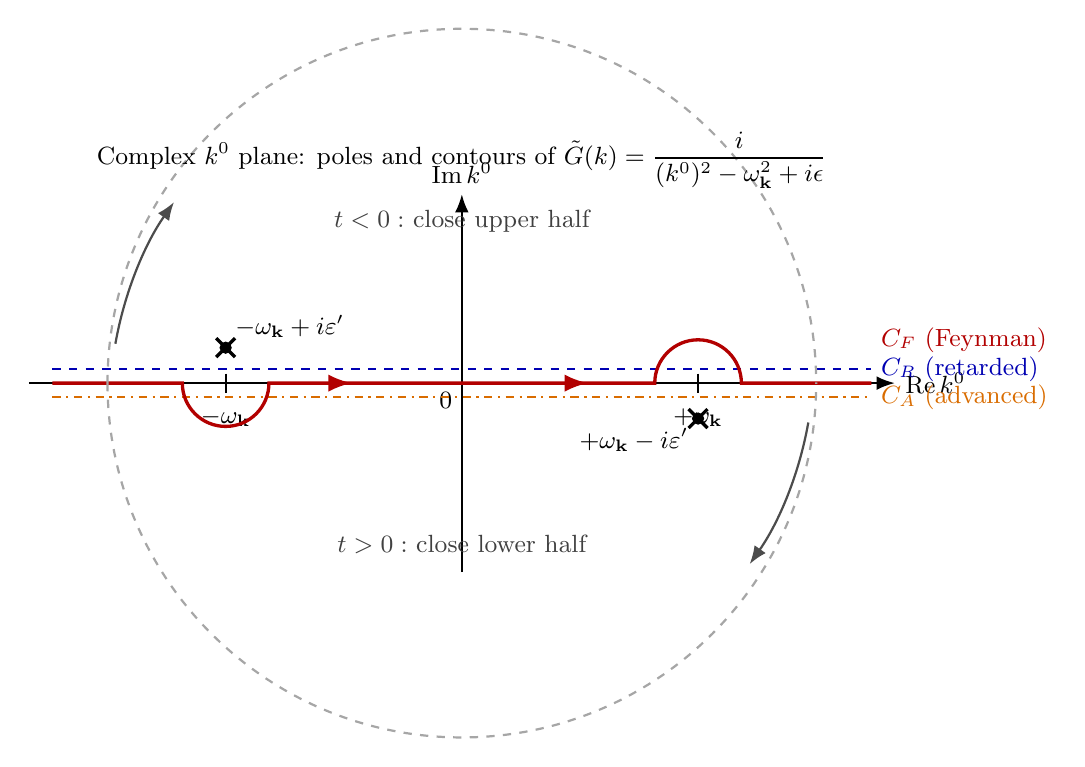
\begin{tikzpicture}[>=Latex, font=\small]

% Coordinate frame: complex k^0 plane
% x axis: Re k^0, y axis: Im k^0
\def\xmin{-5.5}
\def\xmax{5.5}
\def\ymin{-2.4}
\def\ymax{2.4}

% Axes
\draw[->, thick, black] (\xmin,0) -- (\xmax,0)
   node[right] {$\mathrm{Re}\,k^{0}$};
\draw[->, thick, black] (0,\ymin) -- (0,\ymax)
   node[above] {$\mathrm{Im}\,k^{0}$};

% Origin label
\node[below left] at (0,0) {$0$};

% Pole positions
%   negative-energy pole: k^0 = -omega + i*eps'  (upper half)
%   positive-energy pole: k^0 = +omega - i*eps'  (lower half)
\def\omegaX{3.0}
\def\eps{0.45}

% Mass-shell tick marks on real axis
\draw[thick] (-\omegaX,0.12) -- (-\omegaX,-0.12)
   node[below=2pt] {$-\omega_{\mathbf{k}}$};
\draw[thick] ( \omegaX,0.12) -- ( \omegaX,-0.12)
   node[below=2pt] {$+\omega_{\mathbf{k}}$};

% --- Retarded contour: both poles below the line, contour above both
% Drawn as a horizontal line slightly above the real axis
\draw[thick, blue!70!black, dashed]
  (\xmin+0.3,0.18) -- (\xmax-0.3,0.18);
\node[blue!70!black, anchor=west] at (\xmax-0.3,0.18)
  {$C_{R}$ (retarded)};

% --- Advanced contour: both poles above the line, contour below both
\draw[thick, orange!85!black, dash dot]
  (\xmin+0.3,-0.18) -- (\xmax-0.3,-0.18);
\node[orange!85!black, anchor=west] at (\xmax-0.3,-0.18)
  {$C_{A}$ (advanced)};

% --- Feynman contour: along real axis, dipping under negative pole
%     and over positive pole
\def\bump{0.55}    % radius of detour around each pole
\draw[very thick, red!70!black]
  (\xmin+0.3,0)
  -- (-\omegaX-\bump,0)
  arc[start angle=180,end angle=360,radius=\bump]   % go BELOW the negative pole at -omega + i*eps'
  -- (\omegaX-\bump,0)
  arc[start angle=180,end angle=0,radius=\bump]     % go ABOVE the positive pole at +omega - i*eps'
  -- (\xmax-0.3,0);
\node[red!70!black, anchor=west]
  at (\xmax-0.3,0.55) {$C_{F}$ (Feynman)};

% Direction arrows on Feynman contour
\draw[->, very thick, red!70!black]
  (-1.6,0) -- (-1.4,0);
\draw[->, very thick, red!70!black]
  (1.4,0) -- (1.6,0);

% --- Poles: negative-energy in upper half, positive-energy in lower half
% Negative energy pole
\filldraw[black] (-\omegaX, \eps) circle (2pt);
\node[above right] at (-\omegaX, \eps)
  {$-\omega_{\mathbf{k}}+i\varepsilon'$};

% Positive energy pole
\filldraw[black] ( \omegaX,-\eps) circle (2pt);
\node[below left] at ( \omegaX,-\eps)
  {$+\omega_{\mathbf{k}}-i\varepsilon'$};

% Small crosses to mark pole sign distinctly
\draw[black, very thick] (-\omegaX-0.12,\eps+0.12) -- (-\omegaX+0.12,\eps-0.12);
\draw[black, very thick] (-\omegaX-0.12,\eps-0.12) -- (-\omegaX+0.12,\eps+0.12);
\draw[black, very thick] ( \omegaX-0.12,-\eps+0.12) -- ( \omegaX+0.12,-\eps-0.12);
\draw[black, very thick] ( \omegaX-0.12,-\eps-0.12) -- ( \omegaX+0.12,-\eps+0.12);

% Closure-arc indications for t>0 (lower half closure) and t<0 (upper half closure)
% t>0: large dashed arc in lower half
\draw[gray!70, dashed, thick]
  (-4.5,0) arc[start angle=180,end angle=360,radius=4.5];
\node[gray!50!black] at (0,-2.05) {$t>0:$ close lower half};

% t<0: large dashed arc in upper half
\draw[gray!70, dashed, thick]
  (-4.5,0) arc[start angle=180,end angle=0,radius=4.5];
\node[gray!50!black] at (0,2.05) {$t<0:$ close upper half};

% Arrows showing direction of closure (clockwise lower, counterclockwise upper)
\draw[->, gray!60!black, thick]
  (4.4,-0.5) arc[start angle=350,end angle=325,radius=4.5];
\draw[->, gray!60!black, thick]
  (-4.4,0.5) arc[start angle=170,end angle=145,radius=4.5];

% Legend / title at top
\node[anchor=south] at (0,2.35)
  {Complex $k^{0}$ plane: poles and contours of
   $\tilde G(k)=\dfrac{i}{(k^{0})^{2}-\omega_{\mathbf k}^{2}+i\epsilon}$};

\end{tikzpicture}
\end{document}
